\documentclass{article}

% IMPORTANT: Ensure these two packages are correctly included.
\usepackage{tikz}
\usetikzlibrary {calc, positioning, decorations.markings, arrows.meta} 
\usepackage[dvipsnames]{xcolor}
\usepackage{fancyhdr}
\usepackage[left=0.2in, right=0.2in, top=1.5in, bottom=1in]{geometry}
\usepackage{amsmath}
\usepackage{amssymb}
\usepackage{textcomp} 
\usepackage{lipsum}
\newcommand{\vecfive}[5]{\left[ \begin{array}{r} #1\\ #2\\ #3\\ #4 \\#5\end{array}\right]}

\begin{document}

\begin{minipage}[t]{0.45\textwidth}
\centering

% ----JACK AND JOSH 4 NODE VERSION-----
% All options must be correctly bracketed here
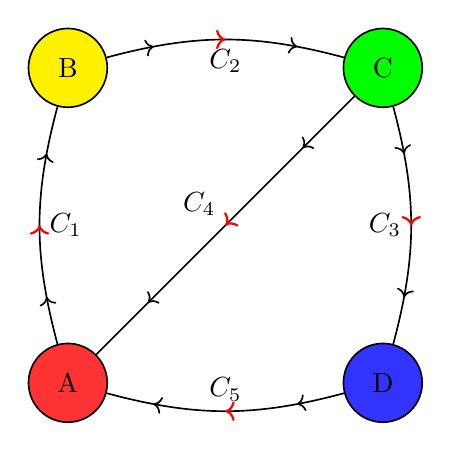
\begin{tikzpicture}[auto, node distance=4cm and 4cm, on grid, semithick, 
    state/.style={ circle, draw, text=black, minimum width=1 cm }]

% Nodes with individual solid colors
\node[state, fill=red!80, draw=black] (A) {A};
\node[state, fill=yellow!100, draw=black] (B) [above =of A] {B};
\node[state, fill=green!100, draw=black] (C) [above right =of A]{C};
\node[state, fill=blue!80, draw=black] (D) [right =of A]{D};

% --- Custom Arrow Style Definition ---
\tikzset{
    three arrows/.style={
        decoration={
            markings,
            mark=at position 0.2 with {\arrow{>}}, 
            mark=at position 0.5 with {\arrow[red, thick]{>}},
            mark=at position 0.8 with {\arrow{>}}
        }, 
        postaction={decorate} 
    }
}
% --------------------------------------

% CORRECT SYNTAX: style name inside square brackets after 'edge'
\path (A) edge[three arrows] [bend left =15] node[right] {$C_1$} (B);
\path (B) edge[three arrows] [bend left =15] node[below] {$C_2$} (C);
\path (C) edge[three arrows] [bend left =15] node[left] {$C_3$} (D);
\path (D) edge[three arrows] [bend left =15] node[above] {$C_5$} (A);
\path (C) edge[three arrows] node[above left] {$C_4$} (A);
\end{tikzpicture}
% ----JACK AND JOSH 4 NODE VERSION-----

\vspace{2cm}

% ----JACK AND JOSH 5 NODE VERSION-----
% All options must be correctly bracketed here
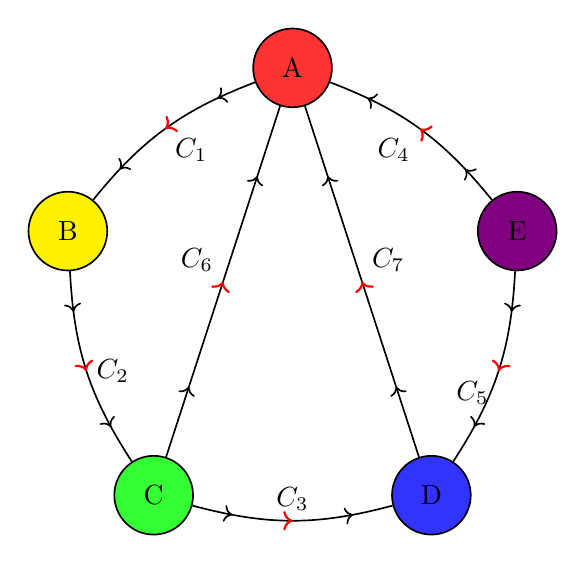
\begin{tikzpicture}[auto, node distance=3 cm and 3cm, on grid, semithick, 
    state/.style={ circle, draw, text=black, minimum width=1 cm }]

%define the radius of the circle and angle from each node
\def\Radius{3cm} 
\def\StartAngle{90} 
\def\AngleStep{72} % 360/5 = 72 degrees

% Nodes with individual solid colors
% Node C (Top) - Angle: 90 + 0*72 = 90
    \node[state, fill=red!80] (A) at (\StartAngle:\Radius) {A}; 
    
    % Node A (Top-Right) - Angle: 90 - 72 = 18 degrees (using 90-72 for a slightly tilted but standard orientation)
    % OR, use 90 - 72 = 18 and 90 + 72 = 162
    \node[state, fill=yellow!100] (B) at (\StartAngle + \AngleStep:\Radius) {B}; % Angle = 18 degrees

    % Node E (Top-Left) - Angle: 90 + 72 = 162 degrees
    \node[state, fill=green!80] (C) at (\StartAngle + 2*\AngleStep:\Radius) {C}; % Angle = 162 degrees

    % Node B (Bottom-Left) - Angle: 162 + 72 = 234 degrees
    \node[state, fill=blue!80] (D) at (\StartAngle + 3*\AngleStep:\Radius) {D}; % Angle = 234 degrees

    % Node D (Bottom-Right) - Angle: 18 + 72 = 90 + 2*72 = 306 degrees
    \node[state, fill=violet!100] (E) at (\StartAngle + 4*\AngleStep:\Radius) {E}; % Angle = 306 degrees

% --- Custom Arrow Style Definition ---
\tikzset{
    three arrows/.style={
        decoration={
            markings,
            mark=at position 0.2 with {\arrow{>}}, 
            mark=at position 0.5 with {\arrow[red, thick]{>}},
            mark=at position 0.8 with {\arrow{>}}
        }, 
        postaction={decorate} 
    }
}
% --------------------------------------

% CORRECT SYNTAX: style name inside square brackets after 'edge'
\path (A) edge[three arrows] [bend right =15] node[below right] {$C_1$} (B);
\path (B) edge[three arrows] [bend right =15] node[right] {$C_2$} (C);
\path (C) edge[three arrows] [bend right =15] node[above] {$C_3$} (D);
\path (E) edge[three arrows] [bend right =15] node[below left] {$C_4$} (A);
\path (E) edge[three arrows] [bend left =15] node[below left] {$C_5$} (D);

\path (C) edge[three arrows] node[above left] {$C_6$} (A);
\path (D) edge[three arrows] node[above right] {$C_7$} (A);
\end{tikzpicture}
% ----JACK AND JOSH 5 NODE VERSION-----
\end{minipage}
\begin{minipage}[t]{0.30\textwidth}
\centering
% ----JACK AND JOSH 4 NODE VERSION-----
% All options must be correctly bracketed here
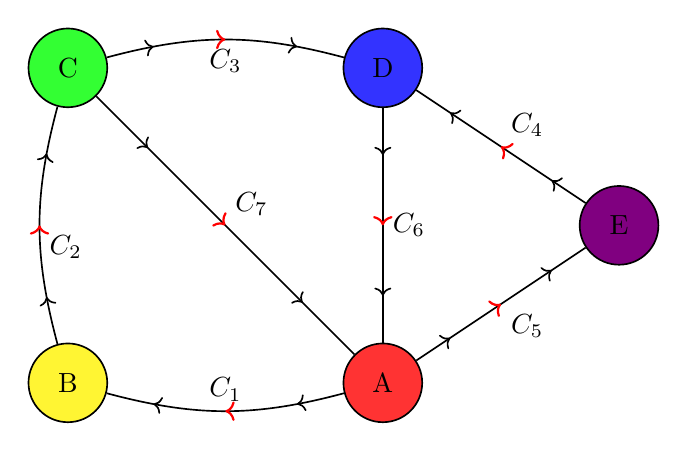
\begin{tikzpicture}[auto, node distance=4cm and 4cm, on grid, semithick, 
    state/.style={ circle, draw, text=black, minimum width=1 cm }]

% Nodes with individual solid colors
\node[state, fill=red!80] (A) at (2.5, 0) {A}; 
\node[state, fill=yellow!80] (B) [left =of A] {B};
\node[state, fill=green!80] (C) [above left =of A] {C};
\node[state, fill=blue!80] (D) [above =of A] {D};
\node[state, fill=violet!100] (E) at ($(A)!0.5!(D) + (3, 0)$) {E};

% --- Custom Arrow Style Definition ---
\tikzset{
    three arrows/.style={
        decoration={
            markings,
            mark=at position 0.2 with {\arrow{>}}, 
            mark=at position 0.5 with {\arrow[red, thick]{>}},
            mark=at position 0.8 with {\arrow{>}}
        }, 
        postaction={decorate} 
    }
}
% --------------------------------------

% CORRECT SYNTAX: style name inside square brackets after 'edge'
\path (A) edge[three arrows] [bend left =15] node[above] {$C_1$} (B);
\path (B) edge[three arrows] [bend left =15] node[below right] {$C_2$} (C);
\path (C) edge[three arrows] [bend left =15] node[below] {$C_3$} (D);
\path (E) edge[three arrows] node[above right] {$C_4$} (D);
\path (A) edge[three arrows] node[below right] {$C_5$} (E);
\path (C) edge[three arrows] node[above right] {$C_7$} (A);
\path (D) edge[three arrows] node[right] {$C_6$} (A);
\end{tikzpicture}
% ----JACK AND JOSH 4 NODE VERSION-----

\vspace{1cm}
% ----JACK AND JOSH 5 NODE VERSION-----
% All options must be correctly bracketed here
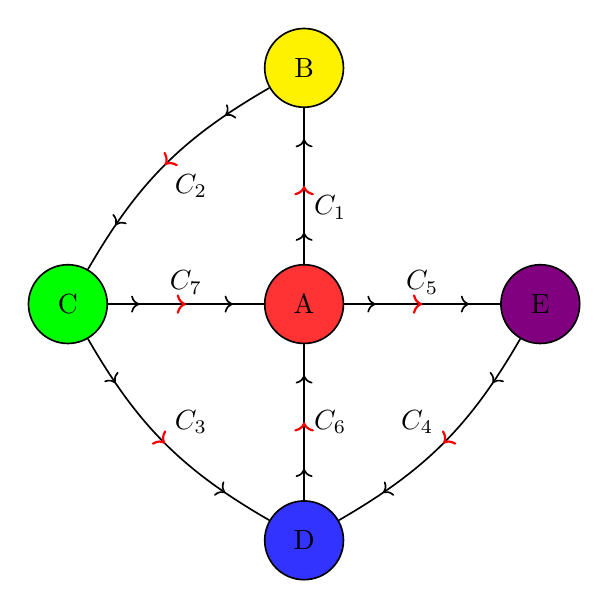
\begin{tikzpicture}[auto, node distance=3 cm and 3cm, on grid, semithick, 
    state/.style={ circle, draw, text=black, minimum width=1 cm }]



% Nodes with individual solid colors
% Node C (Top) - Angle: 90 + 0*72 = 90
\node[state, fill=red!80, draw=black] (A) {A};
\node[state, fill=yellow!100, draw=black] (B) [above =of A] {B};
\node[state, fill=green!100, draw=black] (C) [left=of A]{C};
\node[state, fill=blue!80, draw=black] (D) [below =of A]{D};
\node[state, fill=violet!100, draw=black] (E) [right =of A]{E};
% --- Custom Arrow Style Definition ---
\tikzset{
    three arrows/.style={
        decoration={
            markings,
            mark=at position 0.2 with {\arrow{>}}, 
            mark=at position 0.5 with {\arrow[red, thick]{>}},
            mark=at position 0.8 with {\arrow{>}}
        }, 
        postaction={decorate} 
    }
}
% --------------------------------------

% CORRECT SYNTAX: style name inside square brackets after 'edge'
\path (A) edge[three arrows] node[below right] {$C_1$} (B);
\path (B) edge[three arrows] [bend right =15] node[below right] {$C_2$} (C);
\path (C) edge[three arrows] [bend right =15] node[above right] {$C_3$} (D);
\path (E) edge[three arrows] [bend left =15] node[above left] {$C_4$} (D);
\path (A) edge[three arrows] node[above] {$C_5$} (E);
\path (C) edge[three arrows] node[above] {$C_7$} (A);
\path (D) edge[three arrows] node[right] {$C_6$} (A);
\end{tikzpicture}
% ----JACK AND JOSH 5 NODE VERSION-----
\end{minipage}%

\end{document}